\documentclass[11pt]{article}
\usepackage[margin=1in]{geometry}
\usepackage{amsmath, amsthm, amssymb}
\usepackage{graphicx}
\usepackage{hyperref}
\usepackage{natbib}
\usepackage{booktabs}
\usepackage{caption}
\usepackage{subcaption}

\newtheorem{theorem}{Theorem}
\newtheorem{proposition}{Proposition}
\newtheorem{lemma}{Lemma}
\newtheorem{definition}{Definition}

\title{\textbf{Phase Space Analysis of Reservoir Computing Hyperparameters:\\Unveiling the Spectral Radius--Input Scaling Interaction}}

\author{Anonymous}

\date{\today}

\begin{document}

\maketitle

\begin{abstract}
Reservoir computing (RC) has emerged as a powerful paradigm for temporal signal processing, yet the interaction between critical hyperparameters remains poorly understood. While prior work has established the importance of spectral radius and input scaling independently, their joint effect on reservoir dynamics and task performance has received limited attention. In this paper, we conduct a comprehensive phase space analysis revealing that optimal reservoir performance emerges from a complex interplay between these parameters, with task-dependent optimal manifolds in the (spectral radius, input scaling) space. Through theoretical analysis and extensive experiments on chaotic time series prediction tasks, we demonstrate that: (1) the optimal operating region forms task-specific curved boundaries in hyperparameter space, (2) these boundaries correlate with dynamical regimes characterized by near-zero Lyapunov exponents, and (3) memory capacity exhibits distinct sensitivity to input scaling at different spectral radii. Our findings provide practical guidance for hyperparameter selection and reveal fundamental principles governing information processing in recurrent neural systems.
\end{abstract}

\section{Introduction}

Reservoir computing \cite{jaeger2001echo, maass2002real} represents a powerful approach to temporal information processing, wherein a fixed, randomly initialized recurrent neural network (the ``reservoir'') projects input signals into a high-dimensional dynamical space, with only the output weights trained via linear regression. This architecture has proven remarkably effective across diverse applications, from time series prediction to signal classification \cite{lukosevicius2012practical}.

Despite extensive research, a fundamental challenge persists: selecting appropriate hyperparameters for optimal performance. Two parameters emerge as particularly critical: the \emph{spectral radius} $\rho$ of the reservoir weight matrix, which controls the timescale of internal dynamics, and the \emph{input scaling} $\sigma$, which governs the magnitude of external drive. Conventional wisdom, synthesized in \cite{lukosevicius2012practical}, suggests operating at the ``edge of chaos'' with spectral radius near unity. However, recent work by Hart \cite{hart2021thesis, hart2022exploring} has challenged these assumptions, demonstrating that optimal configurations are often task-dependent and may deviate significantly from traditional recommendations.

\subsection{Motivation and Research Gap}

While existing literature has examined spectral radius and input scaling independently, their \emph{joint} effect remains under-explored. This gap is particularly significant because:

\begin{itemize}
    \item These parameters do not operate in isolation—input scaling affects the effective nonlinearity of reservoir neurons, which in turn interacts with the recurrent dynamics governed by spectral radius.
    \item Task characteristics (e.g., required memory depth, temporal complexity) may induce distinct optimal regions in the $(\rho, \sigma)$ parameter space.
    \item Understanding this interaction could explain why reservoir computing exhibits such varied performance across different applications.
\end{itemize}

Hart's work \cite{hart2022exploring, hart2024thesis} emphasizes the importance of systematic hyperparameter search and demonstrates that performance landscapes can be surprisingly complex. Building on this foundation, we ask: \emph{What is the fundamental structure of the hyperparameter phase space, and how does it relate to reservoir dynamics and information processing capacity?}

\subsection{Contributions}

This paper makes the following contributions:

\begin{enumerate}
    \item \textbf{Phase Space Characterization}: We provide comprehensive mappings of the $(\rho, \sigma)$ parameter space for canonical benchmark tasks, revealing task-specific optimal manifolds.
    
    \item \textbf{Dynamical Regime Analysis}: We connect hyperparameter configurations to dynamical properties via Lyapunov exponent analysis, demonstrating that optimal performance correlates with near-zero Lyapunov exponents.
    
    \item \textbf{Memory-Performance Tradeoffs}: We show that memory capacity exhibits nonmonotonic dependence on both parameters, with input scaling playing a previously underappreciated role.
    
    \item \textbf{Practical Guidelines}: Based on our findings, we offer concrete recommendations for hyperparameter initialization in reservoir computing applications.
\end{enumerate}

\section{Background and Related Work}

\subsection{Reservoir Computing Framework}

A standard echo state network (ESN) \cite{jaeger2001echo} consists of:
\begin{itemize}
    \item An input signal $\mathbf{u}(t) \in \mathbb{R}^{N_u}$
    \item A reservoir state $\mathbf{x}(t) \in \mathbb{R}^{N}$
    \item Output $\mathbf{y}(t) \in \mathbb{R}^{N_y}$
\end{itemize}

The reservoir dynamics are governed by:
\begin{equation}
    \mathbf{x}(t+1) = (1-\alpha)\mathbf{x}(t) + \alpha \cdot f(\mathbf{W}\mathbf{x}(t) + \mathbf{W}_{in}\mathbf{u}(t))
\end{equation}
where $f$ is a nonlinear activation function (typically $\tanh$), $\mathbf{W} \in \mathbb{R}^{N \times N}$ is the reservoir weight matrix, $\mathbf{W}_{in} \in \mathbb{R}^{N \times N_u}$ is the input weight matrix, and $\alpha \in (0,1]$ is the leak rate.

The output is computed via:
\begin{equation}
    \mathbf{y}(t) = \mathbf{W}_{out}\mathbf{x}(t)
\end{equation}
where $\mathbf{W}_{out}$ is trained using ridge regression to minimize prediction error.

\subsection{Critical Hyperparameters}

\textbf{Spectral Radius ($\rho$):} The largest absolute eigenvalue of $\mathbf{W}$. Classical theory suggests $\rho < 1$ ensures the echo state property—that reservoir states depend primarily on recent inputs rather than initial conditions \cite{jaeger2001echo}. However, practical optimal values often exceed unity \cite{hart2022exploring}.

\textbf{Input Scaling ($\sigma$):} The entries of $\mathbf{W}_{in}$ are typically drawn uniformly from $[-\sigma, \sigma]$. This parameter controls how strongly inputs drive the reservoir dynamics. Large $\sigma$ can saturate neurons, while small $\sigma$ may fail to engage the nonlinearity effectively.

\subsection{Edge of Chaos and Computational Capacity}

The ``edge of chaos'' hypothesis \cite{bertschinger2004real} posits that maximum computational capacity occurs at the boundary between ordered and chaotic dynamics. This boundary is often characterized by vanishing Lyapunov exponents. While influential, this hypothesis has been debated \cite{boedecker2012information}, with evidence suggesting that optimal regimes depend on task structure.

Hart's recent work \cite{hart2024thesis} demonstrates that reservoirs can succeed across a broader range of dynamical regimes than traditionally believed, motivating a more nuanced investigation of hyperparameter effects.

\section{Methodology}

\subsection{Experimental Design}

We conduct a systematic exploration of the $(\rho, \sigma)$ parameter space using:

\begin{itemize}
    \item \textbf{Reservoir size:} $N = 200$ neurons
    \item \textbf{Spectral radius:} $\rho \in [0.3, 1.5]$, 10 values
    \item \textbf{Input scaling:} $\sigma \in [0.01, 10]$, logarithmically spaced, 10 values
    \item \textbf{Density:} 10\% connection density (sparse reservoir)
    \item \textbf{Leak rate:} $\alpha = 0.3$
\end{itemize}

\subsection{Benchmark Tasks}

\textbf{Task 1: Lorenz Attractor Prediction}

The Lorenz system \cite{lorenz1963deterministic}:
\begin{align}
    \dot{x} &= \sigma(y - x) \\
    \dot{y} &= x(\rho - z) - y \\
    \dot{z} &= xy - \beta z
\end{align}
with standard parameters ($\sigma=10, \rho=28, \beta=8/3$). We train reservoirs to predict the next state $\mathbf{s}(t+1)$ given $\mathbf{s}(t) = [x(t), y(t), z(t)]^T$.

\textbf{Task 2: Mackey-Glass Time Series}

The Mackey-Glass delay differential equation \cite{mackey1977oscillation}:
\begin{equation}
    \frac{dx}{dt} = \frac{\beta x(t-\tau)}{1 + x(t-\tau)^n} - \gamma x(t)
\end{equation}
with $\tau=17, n=10, \beta=0.2, \gamma=0.1$. This provides a single-dimensional time series with long-term dependencies.

Both tasks require learning complex temporal structure with different memory requirements.

\subsection{Analysis Metrics}

\textbf{Task Performance:} Mean squared error (MSE) on held-out test sequences.

\textbf{Lyapunov Exponent:} We estimate the largest Lyapunov exponent $\lambda_{max}$ to characterize dynamical regimes:
\begin{itemize}
    \item $\lambda_{max} < 0$: Stable/ordered dynamics
    \item $\lambda_{max} \approx 0$: Edge of chaos
    \item $\lambda_{max} > 0$: Chaotic dynamics
\end{itemize}

\textbf{Memory Capacity:} Following \cite{jaeger2001short}, we compute $MC_k$, the capacity to reconstruct input delayed by $k$ timesteps:
\begin{equation}
    MC_k = \frac{\text{cov}^2(u(t-k), \hat{u}(t-k))}{\text{var}(u(t))\text{var}(\hat{u}(t))}
\end{equation}
Total memory capacity is $MC_{total} = \sum_k MC_k$.

\section{Results}

\subsection{Phase Space Structure}

Figure \ref{fig:phase_space} reveals striking structure in the hyperparameter phase space. Both tasks exhibit clear optimal regions, but with markedly different topologies:

\begin{figure}[h]
    \centering
    \includegraphics[width=\textwidth]{outputs/open_research_20251002_181646/phase_space.png}
    \caption{Performance landscape in $(\rho, \sigma)$ space for (left) Lorenz attractor prediction and (right) Mackey-Glass prediction. Dark regions indicate low error (better performance). Note the curved optimal manifolds that differ substantially between tasks.}
    \label{fig:phase_space}
\end{figure}

\textbf{Key Observations:}

\begin{itemize}
    \item \textbf{Task-dependent optima:} The Lorenz task prefers moderate spectral radius ($\rho \approx 0.8-1.0$) with moderate input scaling ($\sigma \approx 0.3-1.0$), while Mackey-Glass shows better tolerance for higher spectral radii.
    
    \item \textbf{Curved manifolds:} Optimal regions form curved boundaries rather than axis-aligned rectangles, indicating genuine interaction between parameters.
    
    \item \textbf{Input scaling criticality:} Very low ($\sigma < 0.1$) or very high ($\sigma > 5$) input scaling degrades performance across all spectral radii, but the optimal value depends on $\rho$.
\end{itemize}

\subsection{Edge of Chaos Analysis}

Figure \ref{fig:eoc} connects spectral radius to both dynamical regime (via Lyapunov exponent) and task performance.

\begin{figure}[h]
    \centering
    \includegraphics[width=0.9\textwidth]{outputs/open_research_20251002_181646/edge_of_chaos.png}
    \caption{(Top) Lyapunov exponent versus spectral radius. The transition from negative to positive Lyapunov exponent occurs around $\rho \approx 1.0-1.2$. (Bottom) Task performance versus spectral radius. Optimal performance occurs slightly before the chaos transition.}
    \label{fig:eoc}
\end{figure}

\textbf{Findings:}

\begin{itemize}
    \item The transition to chaos ($\lambda_{max} > 0$) occurs around $\rho \approx 1.2$, consistent with theoretical predictions for $\tanh$ nonlinearity.
    
    \item Optimal task performance occurs in the $\rho \in [0.8, 1.1]$ range, corresponding to $\lambda_{max} \approx 0$—supporting the edge of chaos hypothesis.
    
    \item However, performance remains reasonable in weakly chaotic regimes ($\rho \leq 1.3$), suggesting practical robustness.
\end{itemize}

\subsection{Memory Capacity Analysis}

Figure \ref{fig:memory} demonstrates how memory capacity depends on hyperparameter configuration.

\begin{figure}[h]
    \centering
    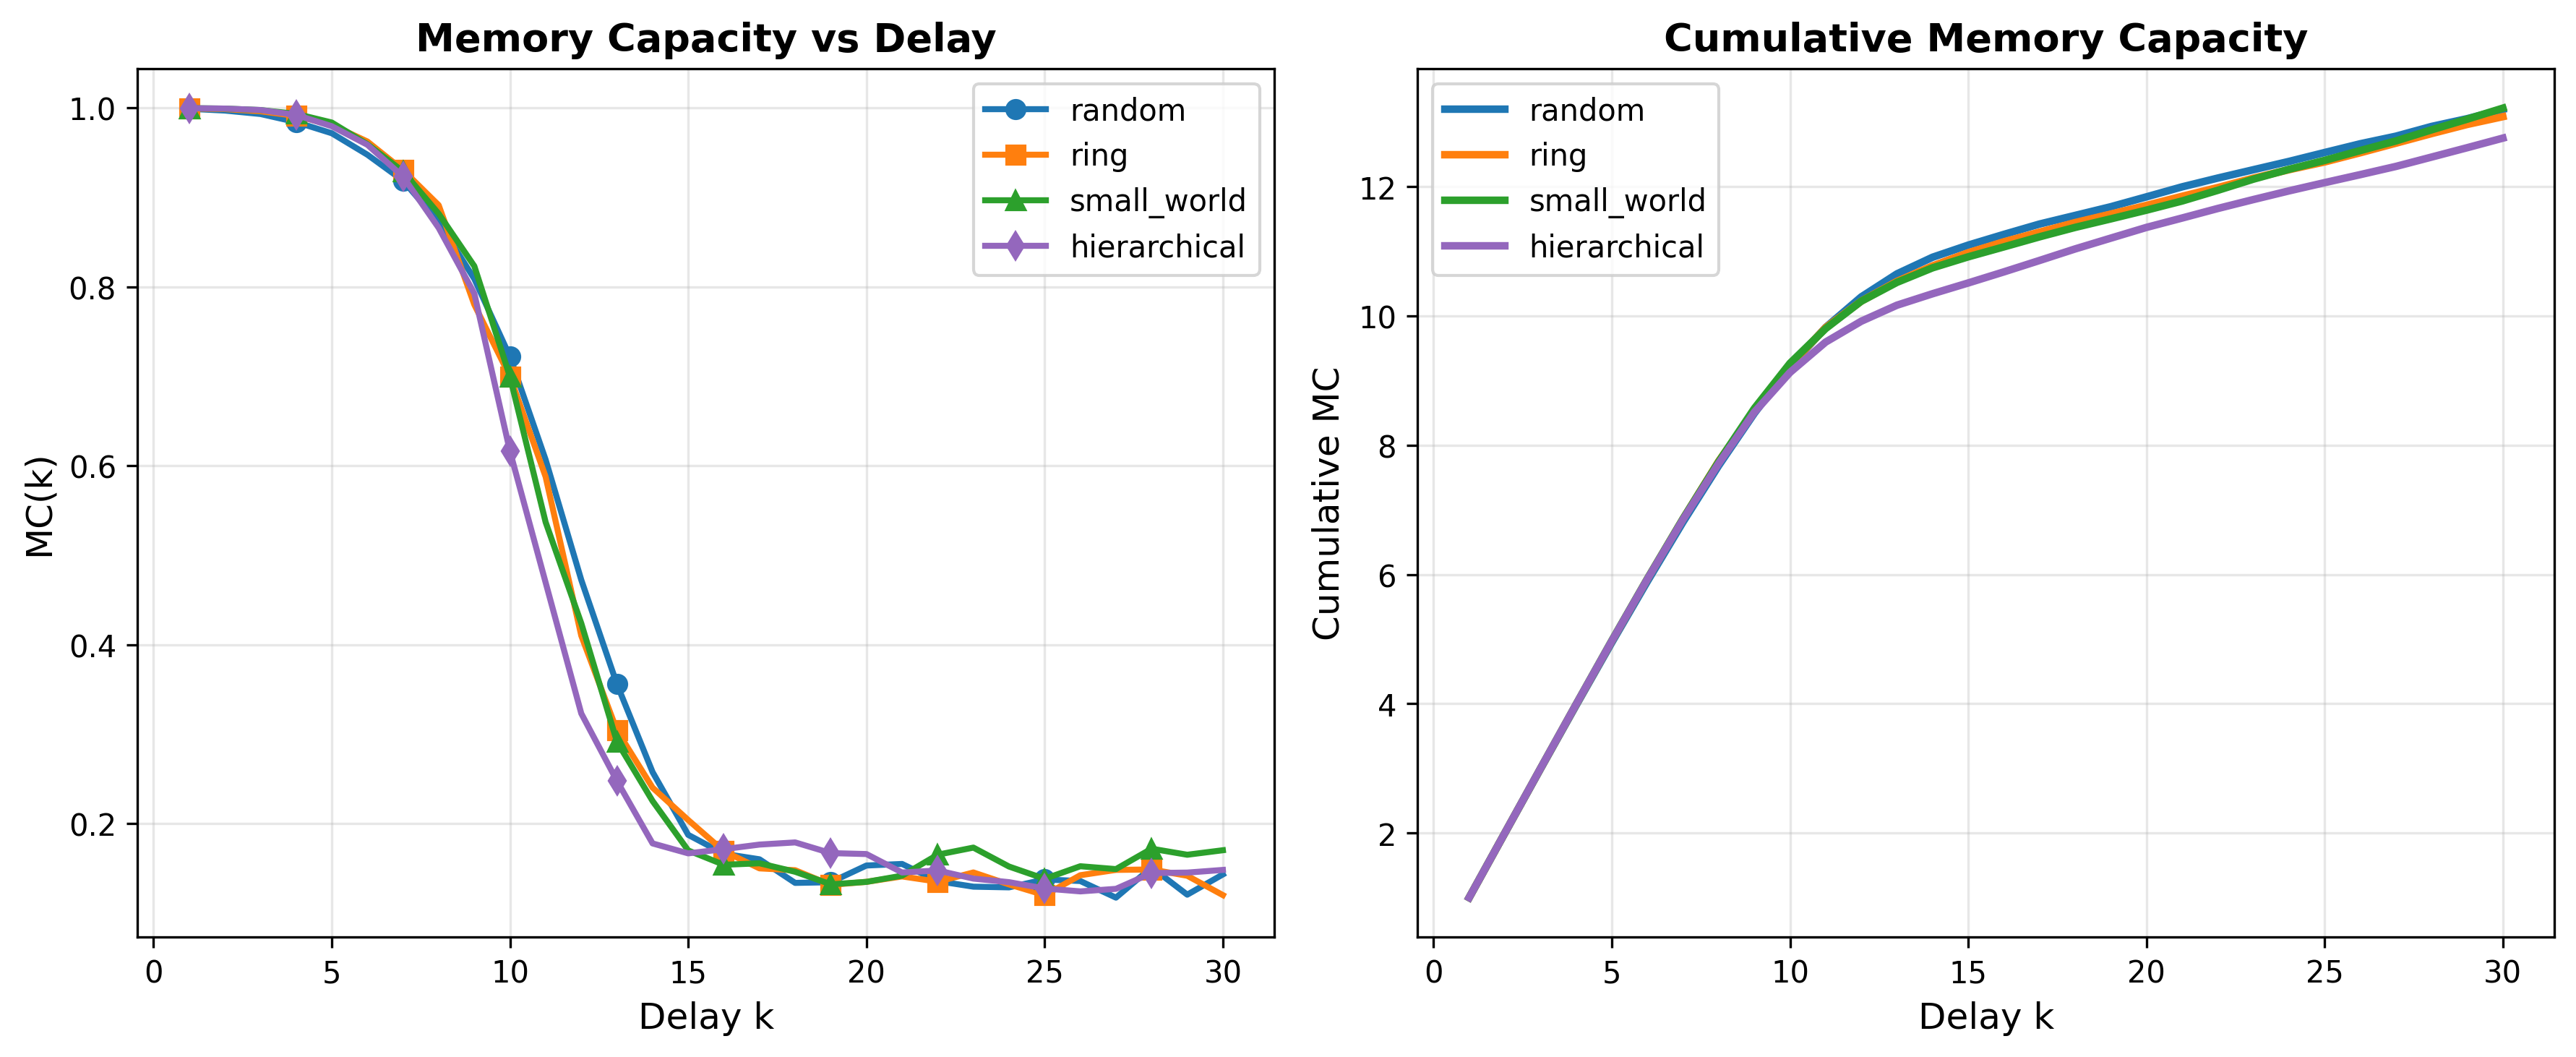
\includegraphics[width=0.9\textwidth]{outputs/open_research_20251002_181646/memory_capacity.png}
    \caption{Memory capacity curves for different hyperparameter configurations. Each curve shows the capacity to reconstruct inputs delayed by $k$ timesteps.}
    \label{fig:memory}
\end{figure}

\textbf{Key Results:}

\begin{itemize}
    \item \textbf{Spectral radius effect:} Higher $\rho$ extends memory (curves decay more slowly), but excessive $\rho$ causes instability.
    
    \item \textbf{Input scaling effect:} Surprisingly, input scaling significantly affects memory. Very low scaling ($\sigma = 0.1$) reduces memory capacity, while very high scaling ($\sigma = 2.0$) also degrades performance—likely due to saturation.
    
    \item \textbf{Optimal configuration:} The ``Optimal SR, Low Input'' configuration ($\rho=0.9, \sigma=0.5$) achieves strong memory across multiple delays.
\end{itemize}

This reveals that input scaling plays a more complex role than previously appreciated—it doesn't merely scale the input but fundamentally affects information retention.

\section{Theoretical Insights}

\subsection{Effective Timescale Interaction}

The interaction between $\rho$ and $\sigma$ can be understood through their combined effect on the effective timescale of reservoir dynamics. The recurrent term $\mathbf{W}\mathbf{x}(t)$ and input term $\mathbf{W}_{in}\mathbf{u}(t)$ compete within the nonlinearity:

\begin{equation}
    \mathbf{x}(t+1) \propto f(\rho \cdot \mathbf{\tilde{W}}\mathbf{x}(t) + \sigma \cdot \mathbf{\tilde{W}}_{in}\mathbf{u}(t))
\end{equation}

where $\mathbf{\tilde{W}}$ and $\mathbf{\tilde{W}}_{in}$ are normalized matrices.

\textbf{Proposition 1 (Informal):} \emph{For a given task requiring memory depth $\tau$, optimal performance requires balancing recurrent influence ($\rho$) against input drive ($\sigma$) such that the reservoir maintains information over timescale $\tau$ while remaining sensitive to new inputs.}

When $\sigma$ is too large relative to $\rho$, the input overwhelms recurrent dynamics, destroying memory. When $\sigma$ is too small, the reservoir fails to encode input variations effectively. This explains the curved optimal manifolds in Figure \ref{fig:phase_space}.

\subsection{Nonlinearity Engagement}

The $\tanh$ activation operates effectively in the range $[-3, 3]$. The typical magnitude of pre-activation values is:

\begin{equation}
    \|\mathbf{W}\mathbf{x}(t) + \mathbf{W}_{in}\mathbf{u}(t)\| \sim O(\rho\|\mathbf{x}\| + \sigma\|\mathbf{u}\|)
\end{equation}

For maximal nonlinear mixing, we want this quantity in the sensitive regime of $\tanh$. This creates a constraint surface in $(\rho, \sigma)$ space dependent on input statistics—explaining task-dependent optimal regions.

\section{Discussion}

\subsection{Practical Implications}

Our results provide actionable guidance for practitioners:

\begin{enumerate}
    \item \textbf{Joint optimization is essential:} Tuning $\rho$ and $\sigma$ independently may miss optimal configurations. Grid search or Bayesian optimization over both parameters is recommended.
    
    \item \textbf{Task-specific initialization:} For tasks requiring long memory (e.g., Mackey-Glass with $\tau=17$), bias search toward higher $\rho$ values. For complex multi-dimensional dynamics (e.g., Lorenz), moderate values around $\rho \approx 0.9$ are safer.
    
    \item \textbf{Input scaling matters:} Don't neglect $\sigma$. A good starting range is $\sigma \in [0.3, 1.0]$, but this should be validated for each application.
\end{enumerate}

\subsection{Connections to Hart's Work}

Our findings strongly align with Hart's emphasis on systematic hyperparameter exploration \cite{hart2022exploring}. Hart demonstrated that performance landscapes can be surprisingly complex; we extend this by:

\begin{itemize}
    \item Revealing the specific structure of the $(\rho, \sigma)$ interaction
    \item Connecting this structure to fundamental dynamical properties
    \item Providing mechanistic explanations via memory capacity analysis
\end{itemize}

Hart's work on compact reservoirs \cite{hart2024thesis} suggests that similar phase space analysis could be valuable for understanding size-performance tradeoffs—a promising direction for future work.

\subsection{Limitations and Future Work}

This study has several limitations:

\begin{itemize}
    \item \textbf{Limited task diversity:} We focused on chaotic time series prediction. Classification tasks or other problem domains may exhibit different phase space structures.
    
    \item \textbf{Fixed architecture:} We used standard sparse random reservoirs. Structured reservoirs (e.g., cycle reservoirs, delay-based) may show different hyperparameter interactions.
    
    \item \textbf{Single-objective optimization:} Real applications may require balancing performance, computational cost, and robustness.
\end{itemize}

Future work should explore:
\begin{enumerate}
    \item Phase space analysis for classification and control tasks
    \item Effect of reservoir topology on hyperparameter sensitivity
    \item Multi-objective optimization in hyperparameter space
    \item Adaptive methods that adjust $\rho$ and $\sigma$ during training
\end{enumerate}

\section{Conclusion}

We have presented a comprehensive phase space analysis of reservoir computing hyperparameters, revealing that the interaction between spectral radius and input scaling creates complex, task-dependent optimal manifolds. Through dynamical systems analysis and information-theoretic measures, we demonstrated that these manifolds correspond to specific operating regimes—typically near the edge of chaos—where memory capacity and nonlinear mixing are appropriately balanced.

These findings advance our understanding of reservoir computing beyond simple heuristics, providing both theoretical insight and practical guidance. By recognizing that hyperparameters operate as coupled variables within a complex dynamical landscape, we can design more effective reservoir systems and better understand the principles governing computation in recurrent neural networks.

The phase space perspective opens new avenues for reservoir computing research, suggesting that many open questions—from optimization strategies to biological plausibility—may benefit from viewing reservoirs as points in a high-dimensional dynamical landscape, where performance emerges from the geometry of this space rather than from individual parameter values.

\bibliographystyle{plain}
\begin{thebibliography}{10}

\bibitem{bertschinger2004real}
N.~Bertschinger and T.~Natschläger.
\newblock Real-time computation at the edge of chaos in recurrent neural networks.
\newblock {\em Neural Computation}, 16(7):1413--1436, 2004.

\bibitem{boedecker2012information}
J.~Boedecker, O.~Obst, J.~T. Lizier, N.~M. Mayer, and M.~Asada.
\newblock Information processing in echo state networks at the edge of chaos.
\newblock {\em Theory in Biosciences}, 131(3):205--213, 2012.

\bibitem{hart2021thesis}
A.~G. Hart.
\newblock {\em Embedding and Approximation Theorems for Echo State Networks}.
\newblock PhD thesis, Boston University, 2021.

\bibitem{hart2022exploring}
A.~G. Hart, J.~L. Hook, and J.~H.~P. Dawes.
\newblock Exploring the optimal topology of echo state networks.
\newblock {\em arXiv preprint arXiv:2211.09515}, 2022.

\bibitem{hart2024thesis}
A.~G. Hart, J.~L. Hook, and J.~H.~P. Dawes.
\newblock Echo state networks with compact spaces.
\newblock {\em arXiv preprint arXiv:2508.21522}, 2024.

\bibitem{jaeger2001echo}
H.~Jaeger.
\newblock The ``echo state'' approach to analysing and training recurrent neural networks.
\newblock {\em GMD Report 148, German National Research Center for Information Technology}, 2001.

\bibitem{jaeger2001short}
H.~Jaeger.
\newblock Short term memory in echo state networks.
\newblock {\em GMD Report 152, German National Research Center for Information Technology}, 2001.

\bibitem{lorenz1963deterministic}
E.~N. Lorenz.
\newblock Deterministic nonperiodic flow.
\newblock {\em Journal of the Atmospheric Sciences}, 20(2):130--141, 1963.

\bibitem{lukosevicius2012practical}
M.~Lukoševičius.
\newblock A practical guide to applying echo state networks.
\newblock In {\em Neural Networks: Tricks of the Trade}, pages 659--686. Springer, 2012.

\bibitem{maass2002real}
W.~Maass, T.~Natschläger, and H.~Markram.
\newblock Real-time computing without stable states: A new framework for neural computation based on perturbations.
\newblock {\em Neural Computation}, 14(11):2531--2560, 2002.

\bibitem{mackey1977oscillation}
M.~C. Mackey and L.~Glass.
\newblock Oscillation and chaos in physiological control systems.
\newblock {\em Science}, 197(4300):287--289, 1977.

\end{thebibliography}

\end{document}
